%!TEX root = ../tesi.tex

\chapter{Test e Risultati}
\label{ch:testerisultati}

In questo capitolo vengono presentati e commentati i test effettuati sui moduli di libreria del progetto.

Nella sezione \ref{sec:strutturatest} viene presentata la struttura dell'impianto di test, sia da lato client che da lato server.
Successivamente, nella sezione \ref{sec:test}, vengono mostrati i risultati dell'esecuzione di alcuni test particolarmente significativi. 
Infine nella sezione \ref{sec:correlate} vi \`e la descrizione di alcune attivit\`a correlate emerse durante lo sviluppo.


\section{Struttura dei test}
\label{sec:strutturatest}
La fase di testing del progetto ha verificato che il funzionamento dei meccanismi implementati all'interno dei moduli esplicati nel capitolo precedente producesse un corretto output visivo.

Oltre a ci\`o questa fase ha avuto l'obbiettivo di riprodurre i test presenti all'interno del progetto \textbf{SF20LiteTestWorld}, che consiste in un modulo di estensione del framework volto a semplificare la gestione delle finestre grafiche nelle applicazioni. Questo modulo \`e in via di sviluppo e per questo non \`e ancora parte integrante delle funzionalit\`a di base offerte dallo \ac{SF}. Tuttavia il codice relativo ad esso \`e disponibile alla stessa fonte della versione del framework indicata al paragrafo \ref{sub:sfsource}.
I test presenti in \textbf{SF20LiteTestWorld} sono stati pensati non solo per verificare la correttezza delle funzionalit\`a, ma anche per mostrare alcune delle capacit\`a del framework stesso.

Per evitare un'eccessiva duplicazione del codice le classi di implementazione dei test, sia lato client che lato server, sfruttano l'ereditariet\`a da una classe genitore comune per condividere tutte le parti comuni.

In figura \ref{f:abstractclient} possiamo vedere la gerarchia delle classi dei client di test. Per implementare un qualsiasi test \`e sufficiente creare una sottoclasse di \texttt{AbstractClient} e implementare al suo interno i metodi astratti della classe genitore. 
\begin{figure}
\begin{center}
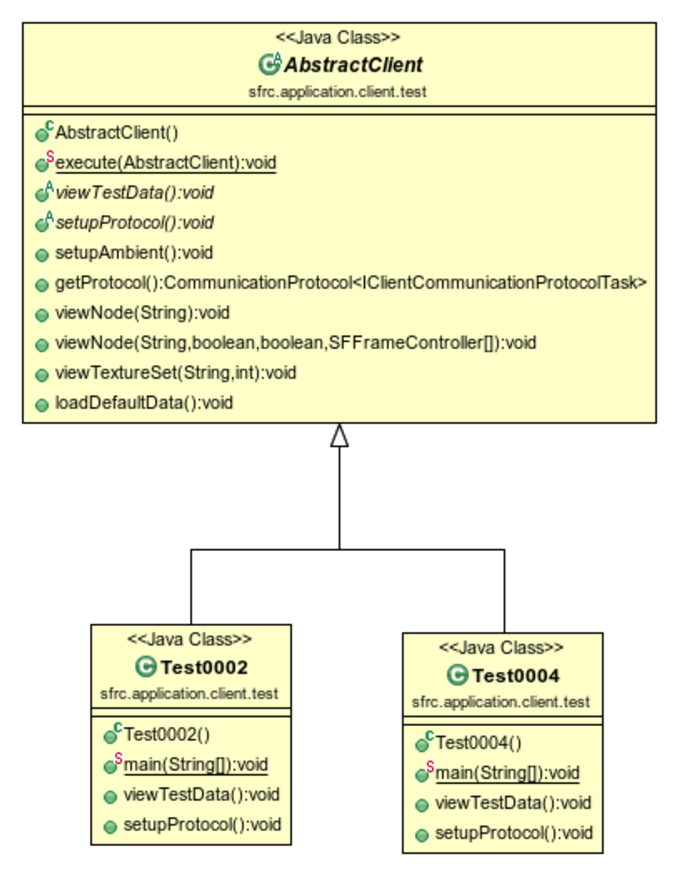
\includegraphics[scale=0.85]{Immagini/abstractclient}
\caption{Gerarchia delle classi di implementazione dei client.\label{f:abstractclient}} 
\end{center} 
\end{figure}
In maniera del tutto simile \`e possibile vedere in figura \ref{f:abstractserver} lo stesso principio applicato per l'implementazione di differenti server di test. Questi, opportunamente configurati, vengono usati per riprodurre le diverse condizioni a cui il client pu\`o essere sottoposto durante la comunicazione, ad esempio generando dei ritardi di risposta o l'assenza di alcuni dati.
\begin{figure}[t]
\begin{center}
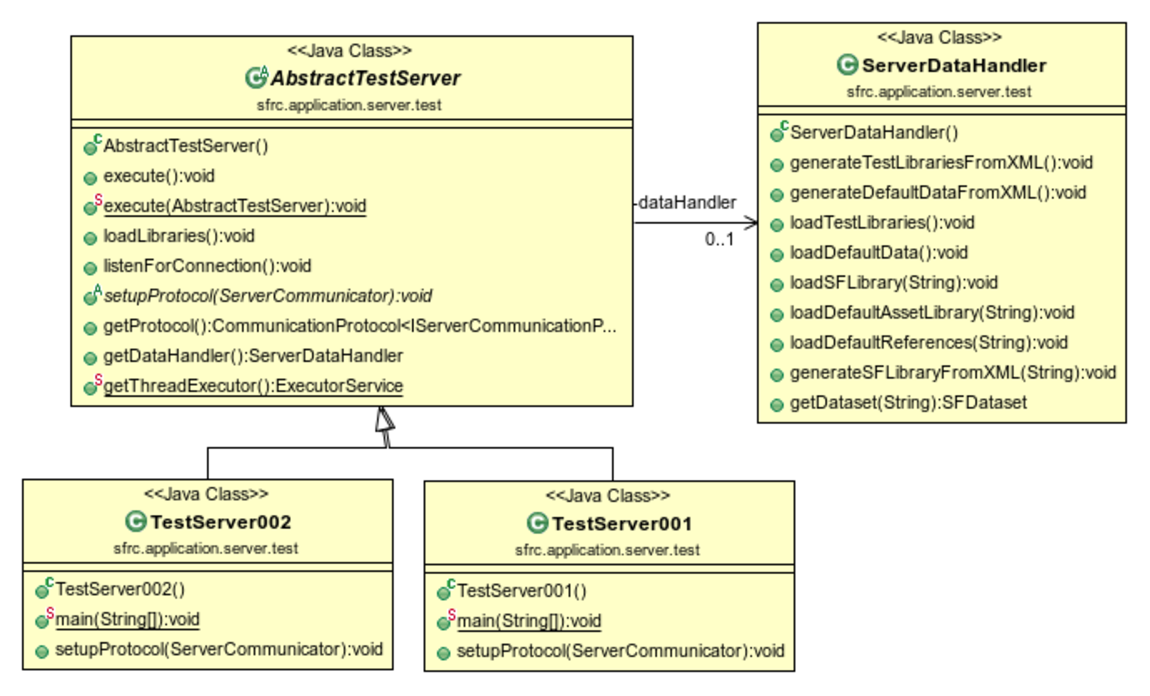
\includegraphics[scale=0.75]{Immagini/abstractserver}
\caption{Gerarchia delle classi di implementazione dei server.\label{f:abstractserver}} 
\end{center} 
\end{figure}
In quest'ultima figura \`e evidenziata la classe \texttt{ServerDataHandler}, la quale si occupa di effettuare la gestione dei dati sul server in esecuzione. Non essendoci la necessit\`a di renderizzare i dati tridimensionali, non \`e richiesta un'infrastruttura centralizzata complessa come quella del DataCenter del framework.

Le classi che implementano i test sono contenute nei package \\\texttt{sfrc.application.client.test} e \texttt{sfrc.application.server.test}.

\section{Test significativi}
\label{sec:test}
Il server di test utilizzato nelle prove descritte di seguito \`e il \textbf{TestServer002} ed \`e stato configurato per avere $3$ secondi di ritardo tra la risposta ad una richiesta ed un'altra. Questa configurazione permette di osservare nel dettaglio la reazione dei meccanismi implementati ad un arrivo progressivo dei dati.

\subsection{Test0006}
Questo test ha l'obbiettivo di visualizzare all'interno di una finestra, tre oggetti che condividono una geometria dalla forma di fungo e su cui sono applicate delle texture. Sia la geometria che le texture sono generate proceduralmente durante l'esecuzione usando la capacit\`a di calcolo della \ac{GPU}.
\begin{figure}%[t]
\begin{center}
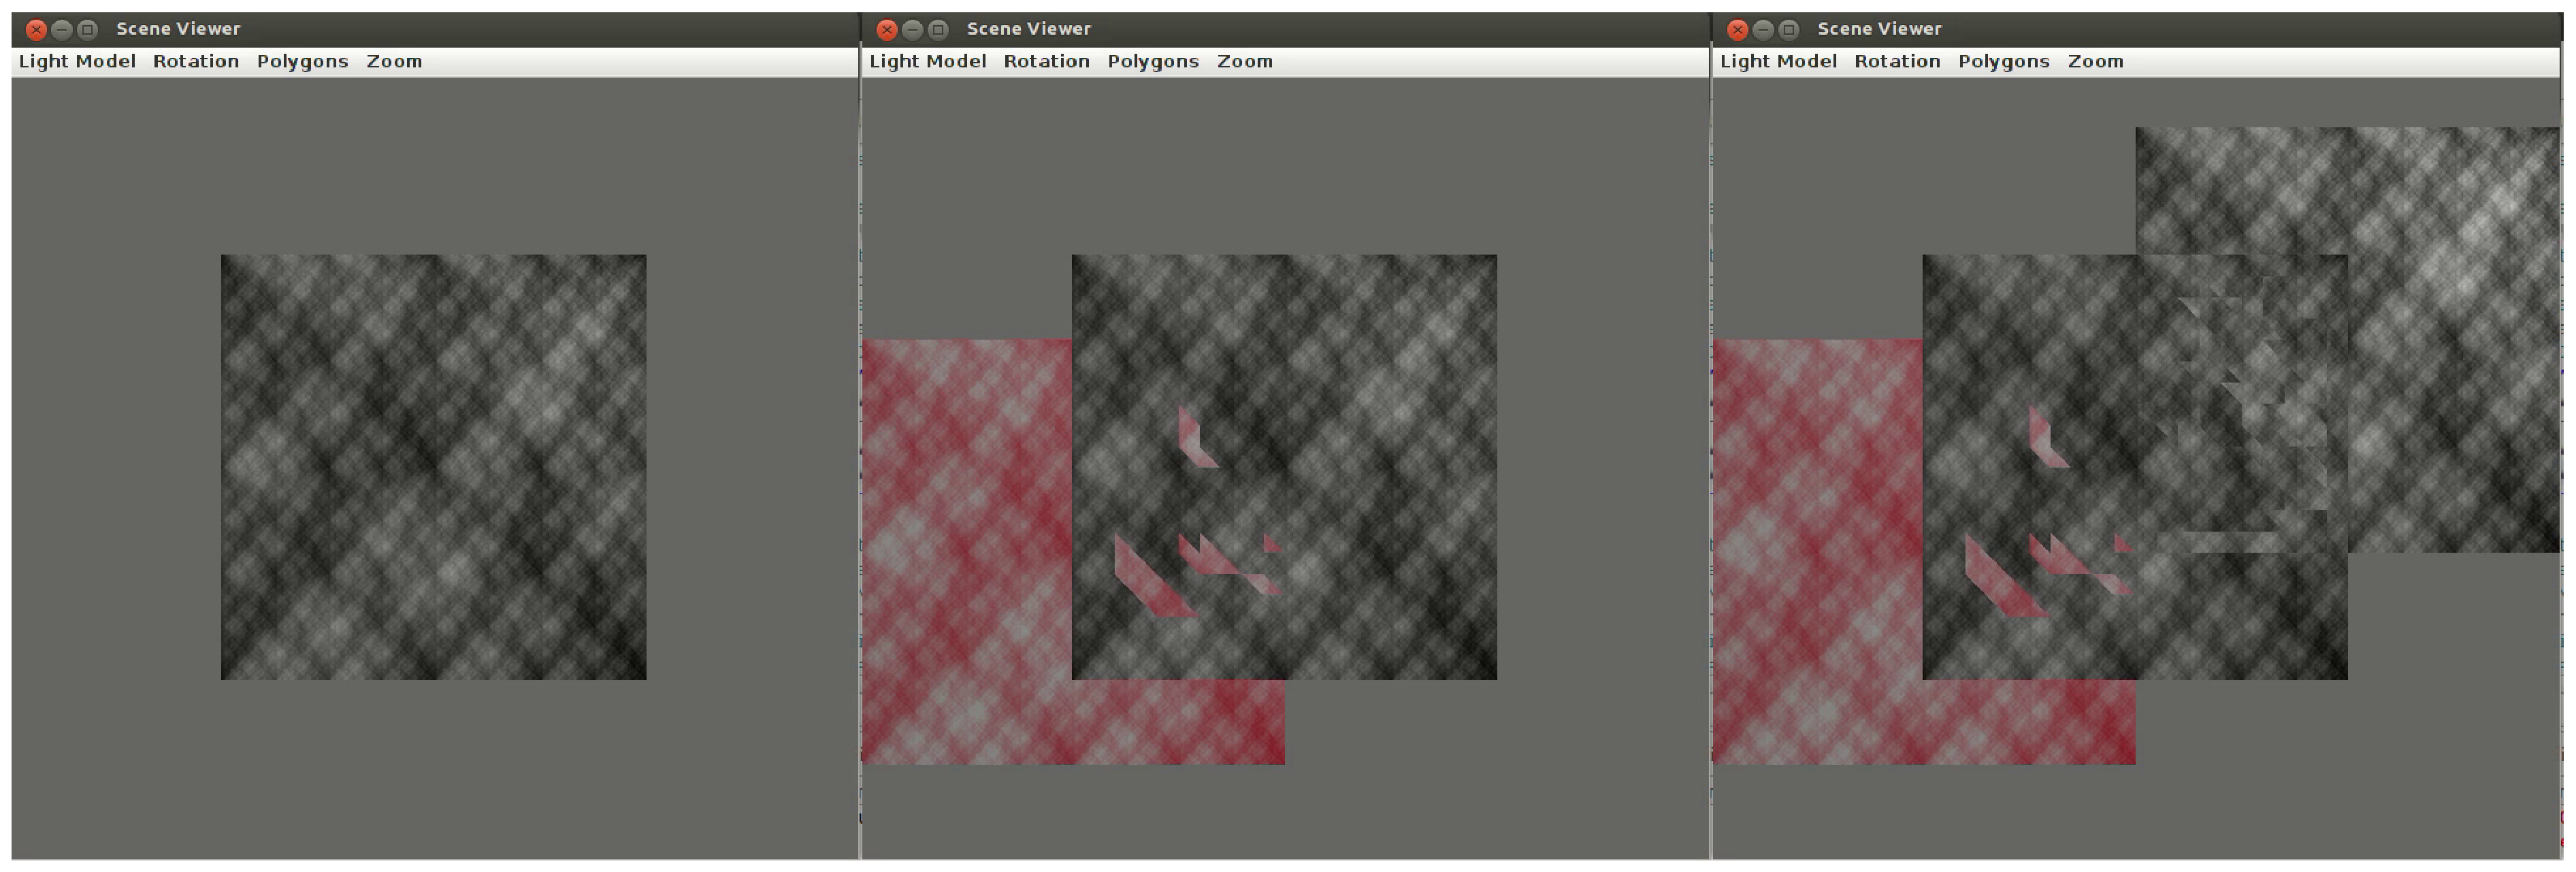
\includegraphics[width=\textwidth]{Immagini/test0006/test0006-wall1}
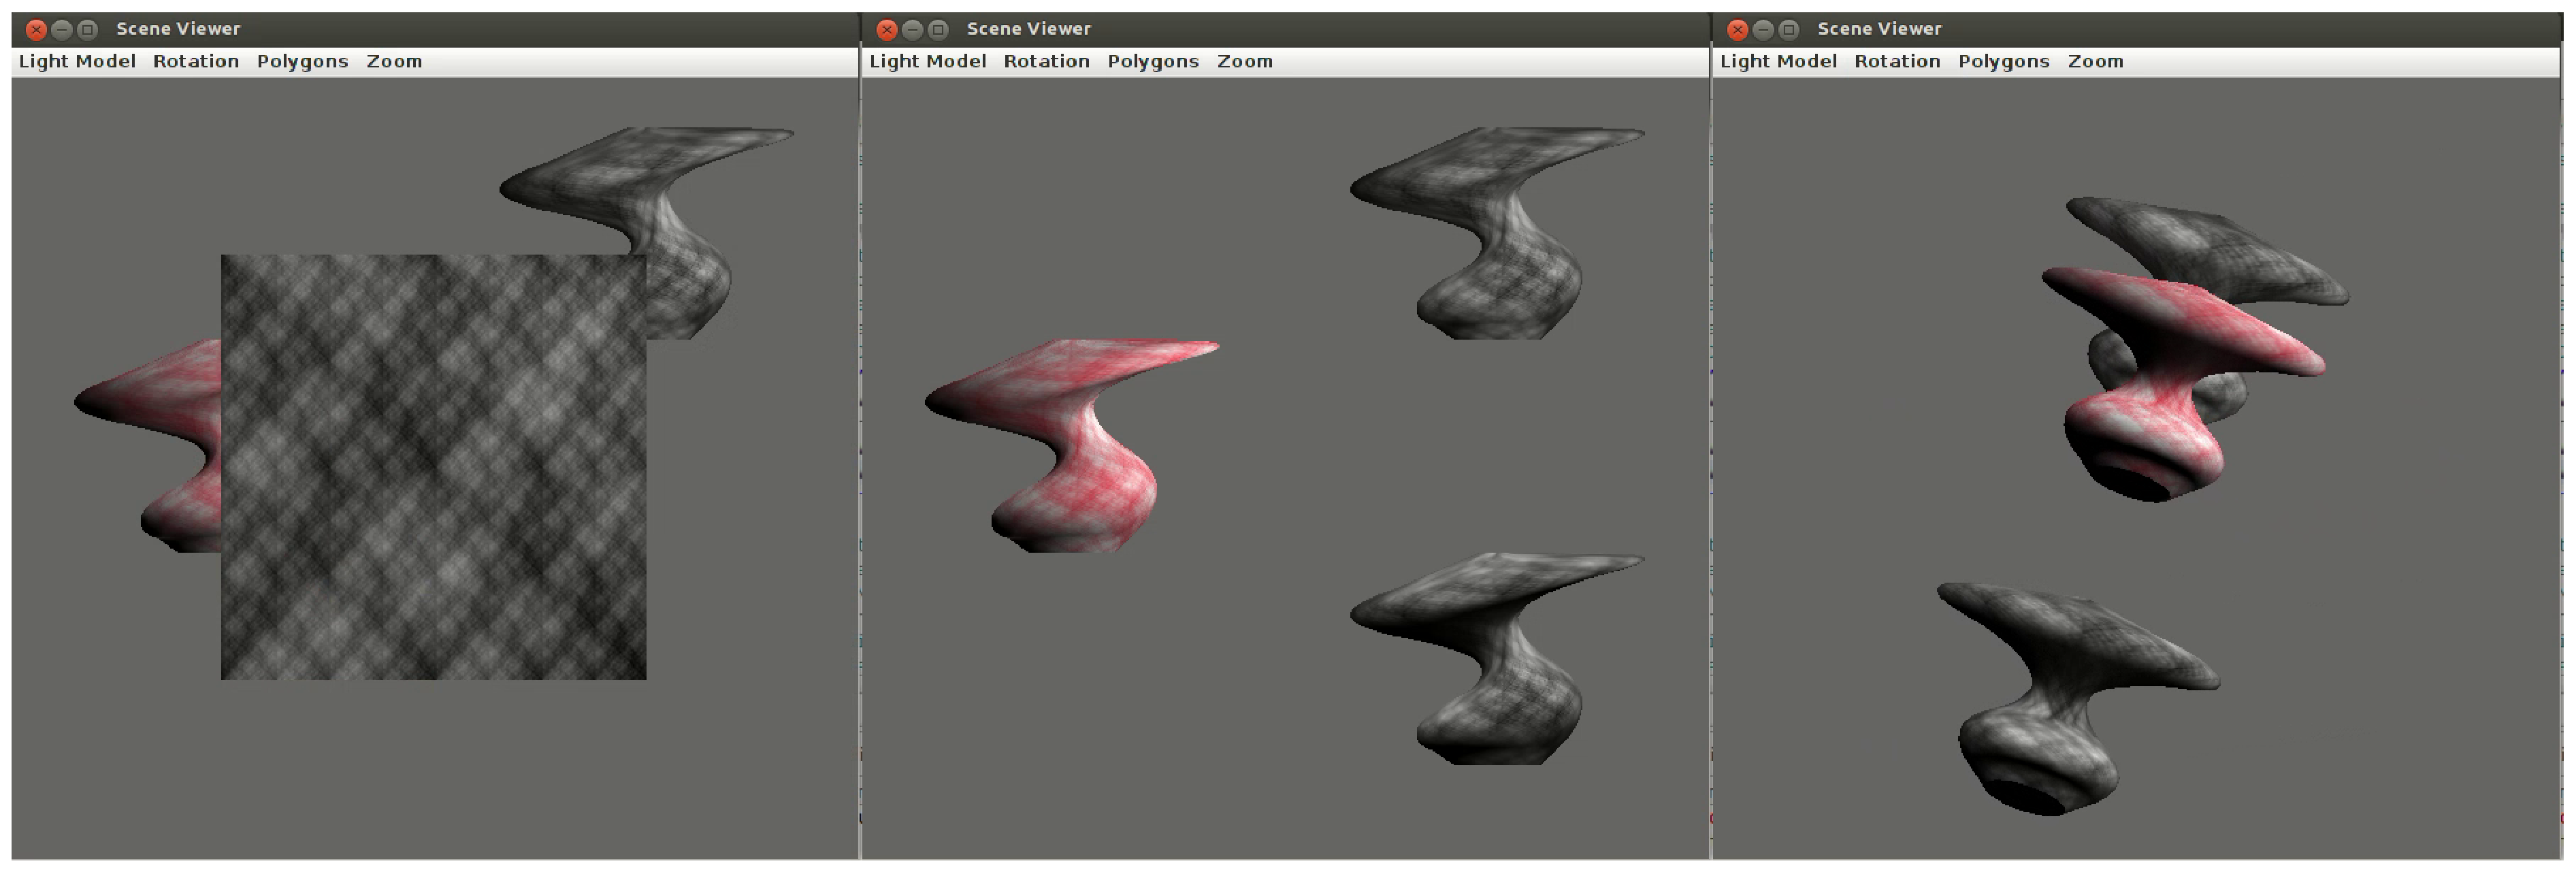
\includegraphics[width=\textwidth]{Immagini/test0006/test0006-wall2}
\caption{Fotogrammi estratti dall'esecuzione del test Test0006. \label{f:test0006-wall}} 
\end{center} 
\end{figure}
In figura \ref{f:test0006-wall} viene mostrata una sequenza di fotogrammi dell'esecuzione del test: al lancio dell'applicazione (fig.\ref{f:test0006-wall} in alto a sinistra) la scena richiesta viene temporaneamente sostituita con un'altra che contiene un semplice cubo texturizzato. 
Al loro arrivo, i dati della scena reale che contengono i riferimenti ai tre oggetti vengono analizzati generando la richiesta degli oggetti verso il server. Nel frattempo ognuno di essi viene sostituito con un cubo posto al centro della scena. La sostituzione non genera un cambiamento visibile in quanto i tre cubi sono sovrapposti e posizionati esattamente come quello contenuto nella scena sostitutiva.

Quando i dati del primo oggetto vengono ricevuti (fig.\ref{f:test0006-wall} in alto al centro) vengono immediatamente applicati alla scena: possiamo notare il cambiamento di colore e la traslazione di un cubo verso sinistra. 
L'oggetto non cambia forma perch\'e il pacchetto di informazioni contiene un riferimento alla geometria ``fungo'' generica ancora non presente e per cui viene generata una richiesta. 
Nel fotogramma successivo (fig.\ref{f:test0006-wall} in alto a destra) vediamo gli effetti dell'arrivo del pacchetto di informazioni relativo al secondo oggetto: un altro cubo viene traslato, stavolta verso destra. 
L'informazione sulla geometria ``fungo'' non \`e ancora arrivata, ma non viene generata una nuova richiesta dato che il sistema ha gi\`a una richiesta pendente, l'oggetto viene invece registrato per un update della geometria.
Nel quarto fotogramma (fig.\ref{f:test0006-wall} in basso a sinistra), viene ricevuta la geometria e tutti gli oggetti che si erano registrati per un update vengono aggiornati. Non avendo ancora ricevuto i dati relativi al terzo oggetto, esso rimane nella sua forma sostitutiva. Questo accade a causa del parallelismo dei processi che effettuano le richieste, il quale consente di non dover necessariamente ricevere i dati in un ordine specifico.
Nella penultima immagine (fig.\ref{f:test0006-wall} in basso al centro) si vede l'aggiornamento visivo all'arrivo delle informazioni sul terzo oggetto. Avendo gi\`a ricevuto i dati della geometria essa viene applicata immediatamente insieme alla traslazione. Nell'ultimo fotogramma vediamo la scena finale ruotata dai controlli della finestra client. Per effettuare la navigazione della scena non \`e pi\`u necessario richiedere altri dati al server e le connessioni vengono chiuse. In figura \ref{f:schemadati} sono rappresentate le relazioni tra i dati durante l'esecuzione del test.
\begin{figure}
\begin{center}
\includegraphics[width=\textwidth]{Immagini/schemadati}
\caption{Schema delle relazioni interne tra i dati del Test0006.\label{f:schemadati}} 
\end{center} 
\end{figure}

Per non appesantire la precedente descrizione si \`e omesso che durante l'esecuzione sono stati richiesti e trasferiti anche i dati relativi alle texture da applicare ai modelli. La transizione non \`e direttamente visibile dato che le texture sostitutive hanno la stessa trama e non sono visivamente distinguibili.

\subsection{Test0019}
Questo test prevede la visualizzazione di un oggetto avente geometria a fungo a cui viene applicata una texture e una \textit{bump map}\footnote{Una bump map \`e un particolare tipo di texture che viene utilizzata tramite la tecnica del \textit{Bump Mapping}. Questa tecnica si serve delle informazioni della bump map per descrivere la variazione da applicare al vettore normale di ogni punto di una superficie a cui \`e applicata. Ci\`o permette di ottenere l'effetto visivo di superfici irregolari senza spostare i vertici della superficie stessa}. Anche in questo caso sia la geometria che le texture sono ottenute proceduralmente attraverso il rendering della \ac{GPU}.
\begin{figure}%[t]
\begin{center}
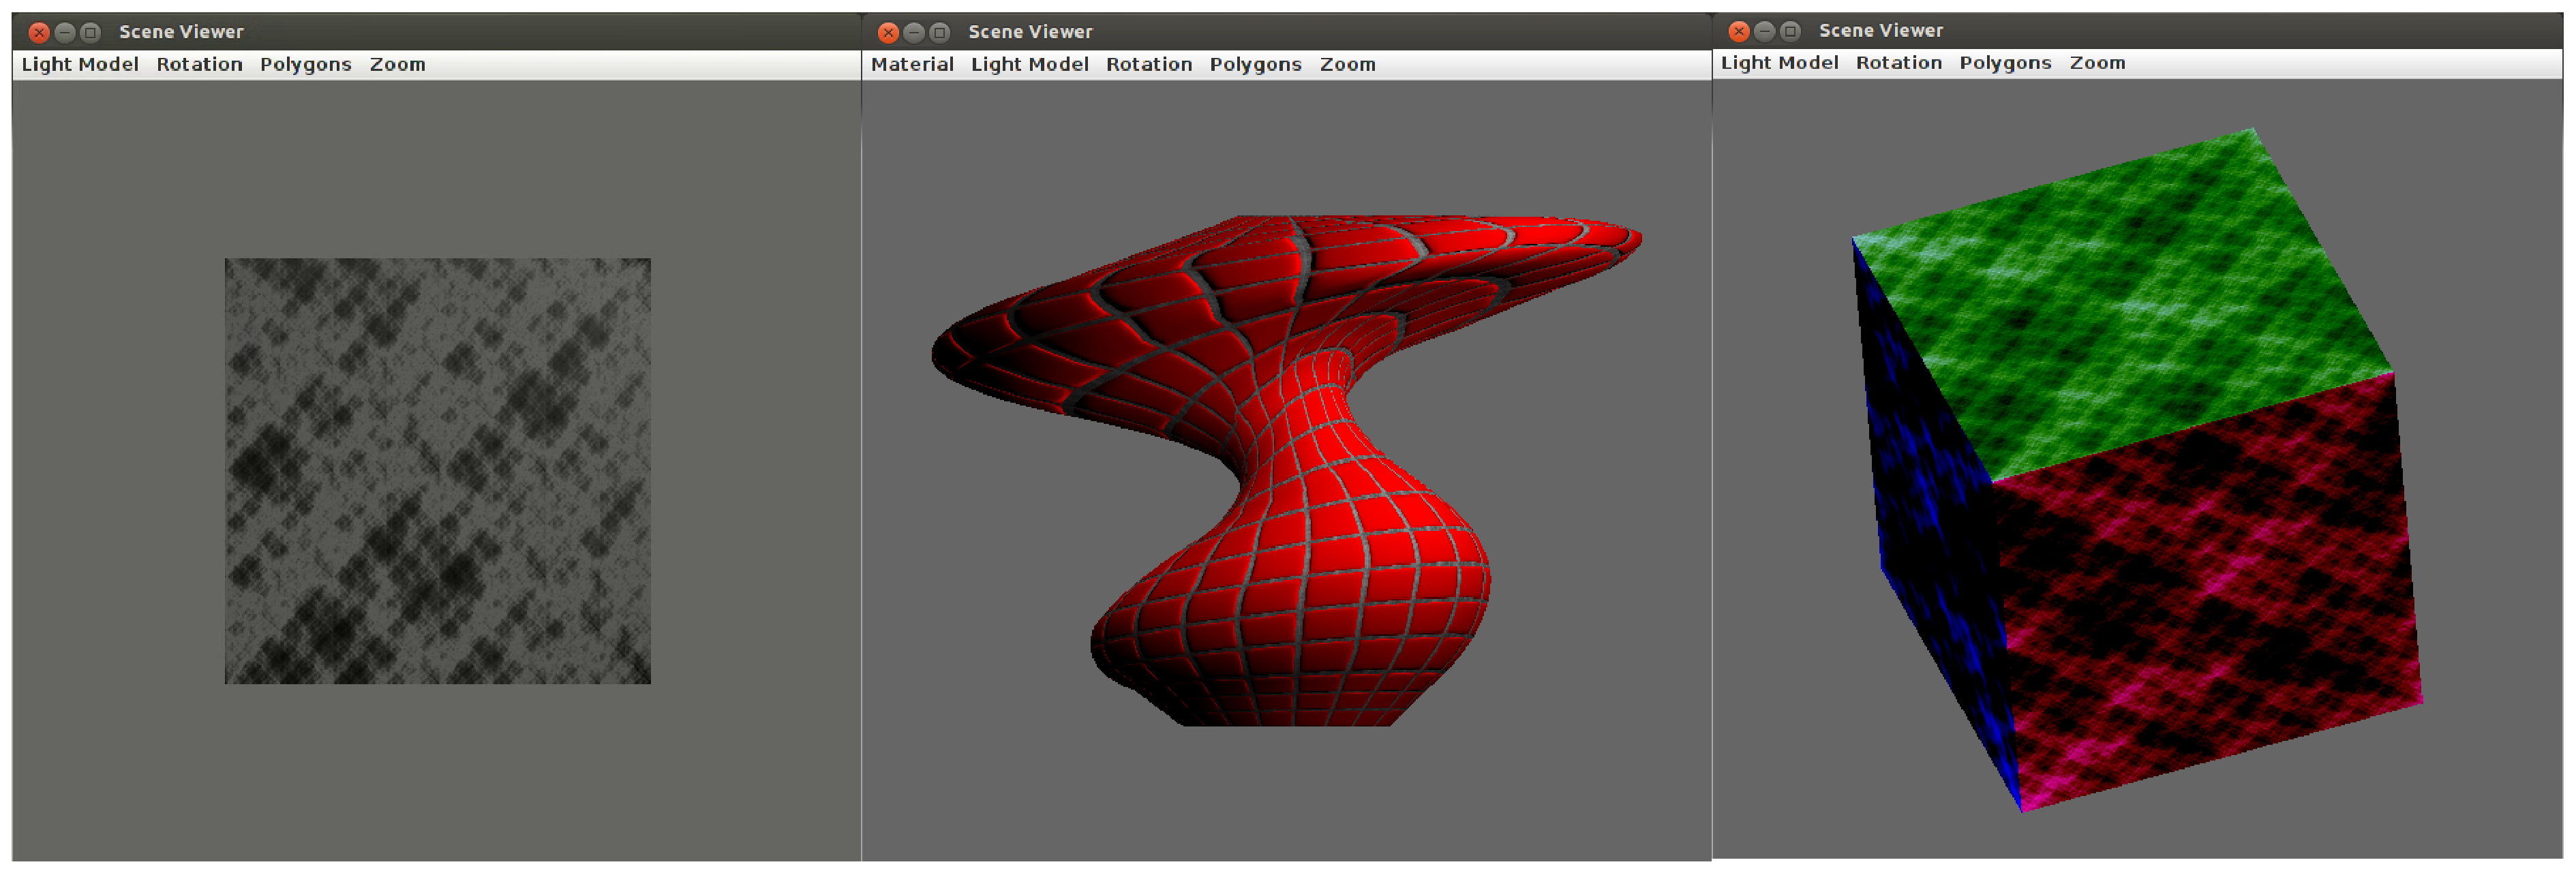
\includegraphics[width=\textwidth]{Immagini/test0019/test0019-wall1}
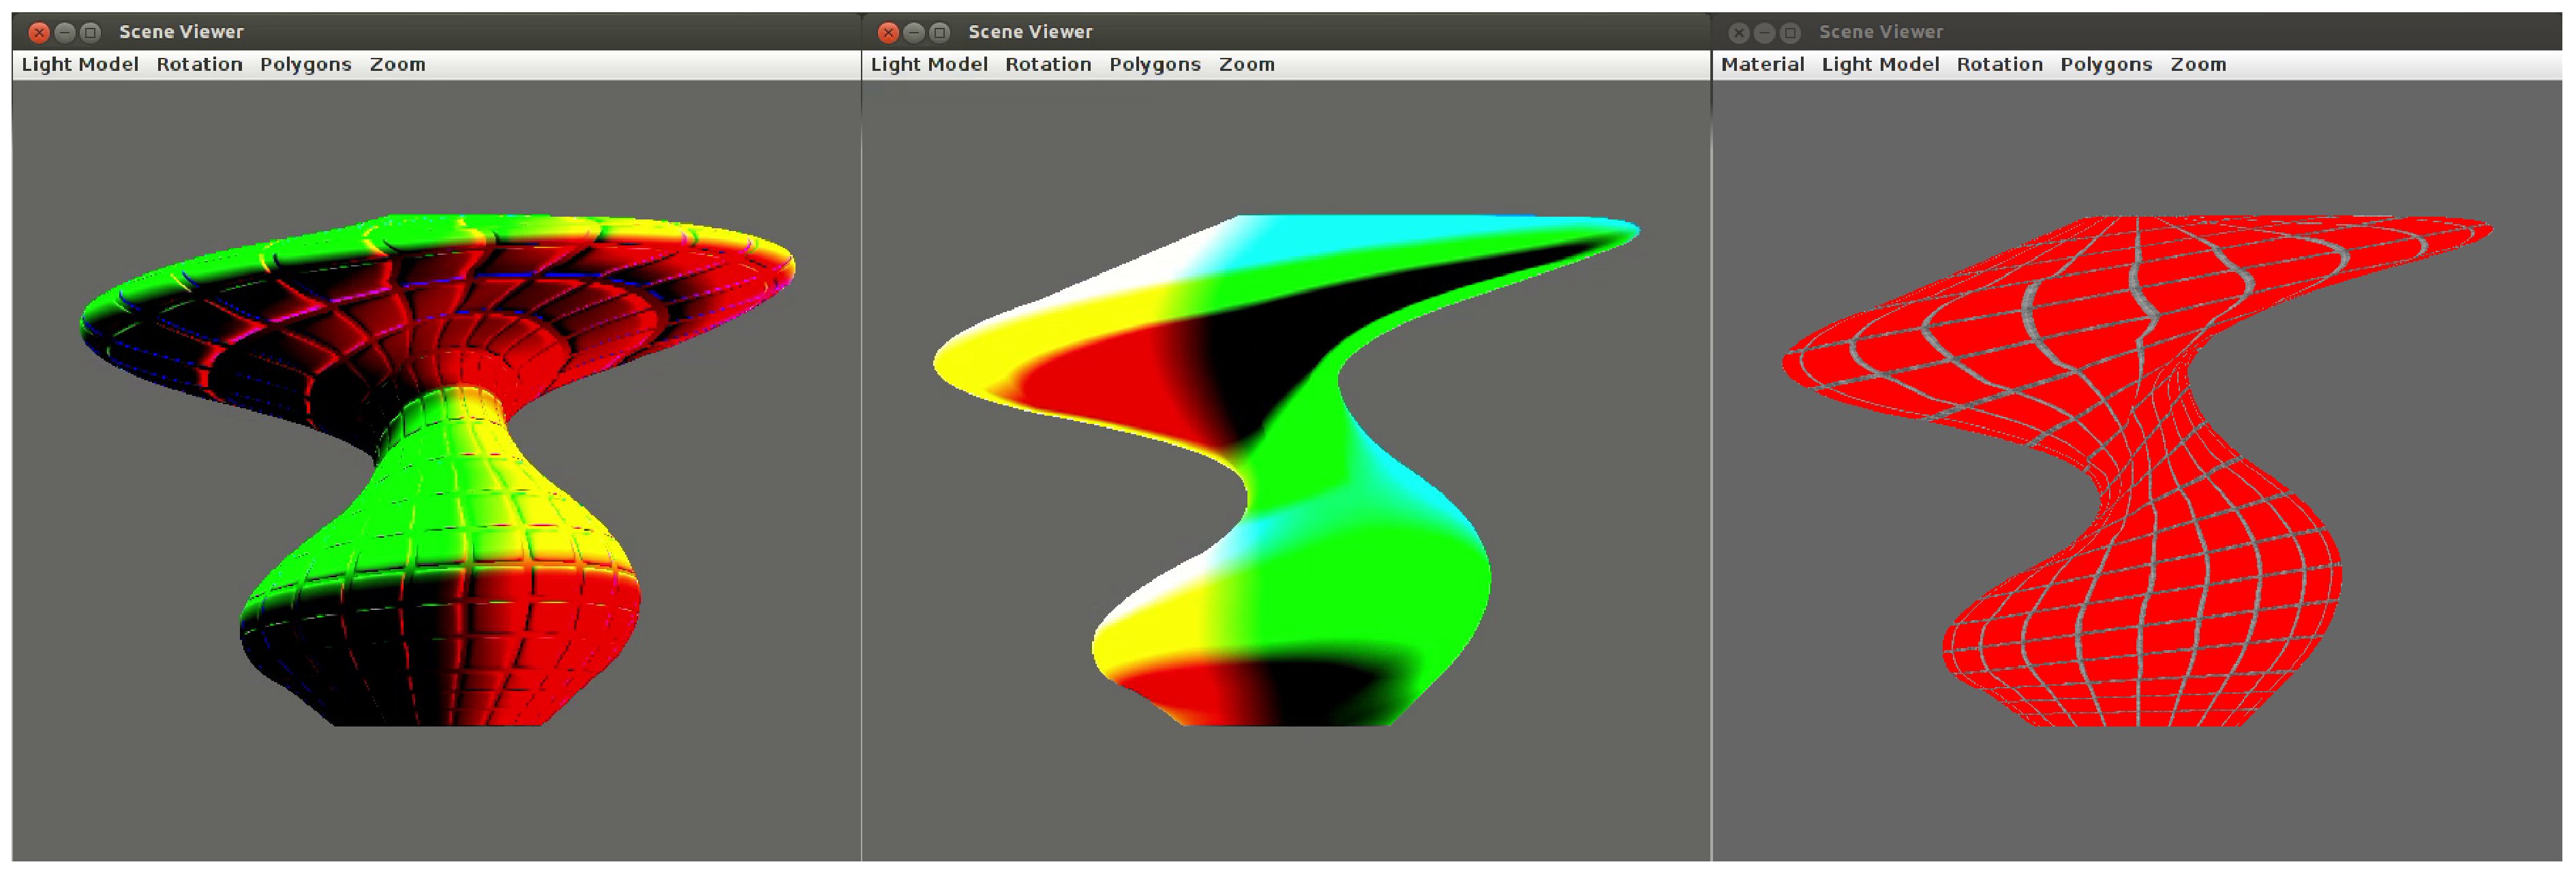
\includegraphics[width=\textwidth]{Immagini/test0019/test0019-wall2}
\caption{Fotogrammi estratti dall'esecuzione del test Test0019. \label{f:test0019-wall}} 
\end{center} 
\end{figure}
Nei primi due fotogrammi in alto a sinistra della figura \ref{f:test0019-wall} vediamo le immagini della geometria sostitutiva (il cubo) e dell'oggetto reale della scena richiesta, anche in questo caso un fungo. L'obbiettivo del test \`e verificare che l'effetto di Bump Mapping venga applicato correttamente alla geometria del fungo una volta che essa viene ottenuta tramite la connessione.
Nella seconda immagine si pu\`o infatti notare l'effetto ``piastrellato'' sulla superficie dell'oggetto. Sebbene dalla prima immagine non sia ben distinguibile, anche il cubo sostitutivo fa uso di questa tecnica: nel terzo fotogramma (fig.\ref{f:test0019-wall} in alto a destra) esso viene disegnato in modo che ogni punto della sua superficie sia di un colore diverso in base alla direzione del vettore normale al punto stesso. Le facce, pur essendo piatte, non hanno un colore uniforme mostrando la corretta applicazione della tecnica. Il quarto fotogramma (fig.\ref{f:test0019-wall} in basso a sinistra) illustra lo stesso effetto applicato al fungo: a un colore diverso sulla superficie corrisponde una normale puntata in una diversa direzione. Gli ultimi due fotogrammi mostrano rispettivamente la geometria finale, colorata in base alla direzione della luce senza tener conto delle normali, e la geometria colorata applicando la texture in modo piatto senza illuminazione.

\begin{figure}
\begin{center}
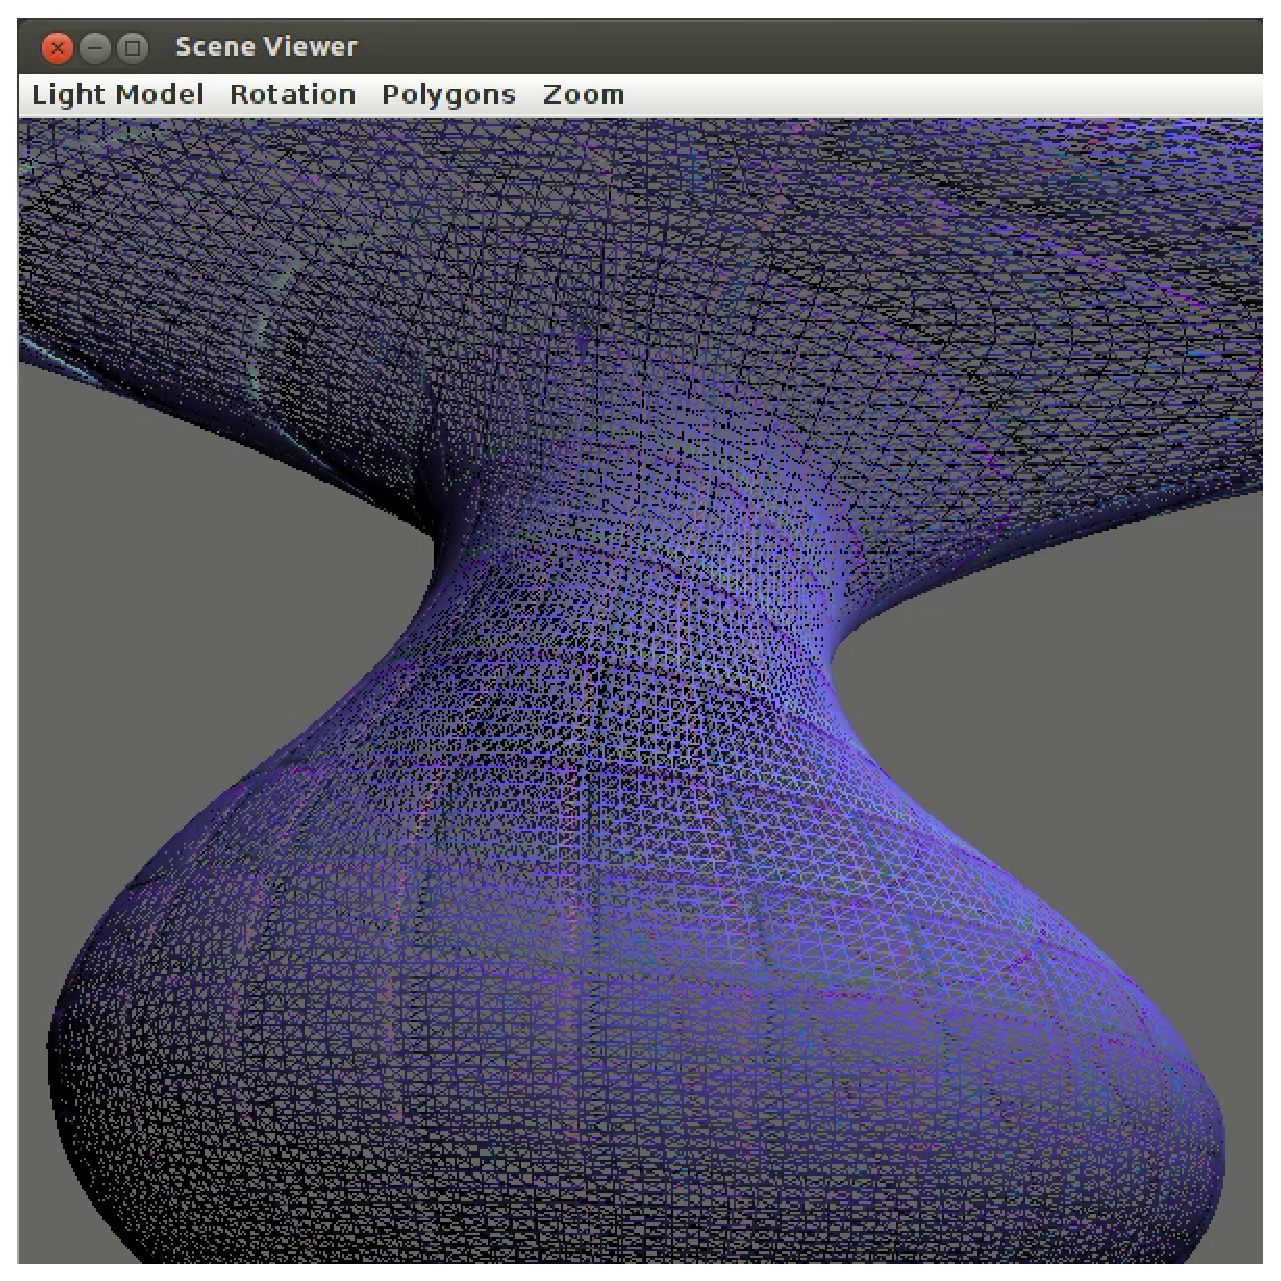
\includegraphics[width=10cm]{Immagini/test0019/test0019-tessel}
\caption[Tassellazione della geometria usata nel Test0019.]{Particolare di un fotogramma estratto dall'esecuzione del test Test0019, \`e posta in evidenza la tassellazione in triangoli operata sul modello del fungo. \label{f:test0019-tessel}} 
\end{center} 
\end{figure}
Come esplicato la tecnica applicata non effettua una reale traslazione dei vertici della geometria, in figura \ref{f:test0019-tessel} vediamo messo in risalto questo particolare grazie ad uno zoom ravvicinato. Con questa immagine possiamo vedere anche il livello di tassellazione della geometria generata dalla pipeline programmabile.

\section{Attivit\`a correlate}
\label{sec:correlate}
La variet\`a dei contenuti dei test di riferimento ha reso necessario un lavoro aggiuntivo dedicato alla creazione di un insieme di Dataset sostitutivi da inserire nella libreria di oggetti di default, usati come rimpiazzo temporaneo.
Questa libreria \`e stata realizzata progressivamente durante l'implementazione dei test, quando si rendeva necessaria la costruzione di un Dataset specifico e quelli gi\`a realizzati erano di tipo incompatibile.
Queste incompatibilit\`a dipendono da ci\`o che i Dataset rappresentano: geometrie, texture, etc. 

Oltre a ci\`o \`e stato necessario implementare un metodo pratico per definire la lista di Dataset sostitutivi con cui effettuare gli scambi. La sola creazione della classe \texttt{SFDatasetReplacement} rendeva necessario definire a runtime la lista, che poteva essere memorizzata solamente in un file binario non leggibile ne modificabile senza un apposito tool. Per risolvere il problema \`e stato modificato il modulo di lettura/scrittura dei file xml preesistente nel framework, aggiungendo la capacit\`a di codificare e decodificare i dati contenuti in un \texttt{SFDatasetReplacement}. 
La lista dei sostituti \`e cos{\`\i} editabile a mano modificando un file testuale xml chiaramente leggibile (figura \ref{f:listaxml}).

\begin{figure}
\begin{center}
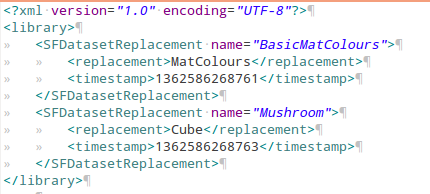
\includegraphics[width=10cm]{Immagini/listaxml}
\caption{File xml della lista di sostituzione.\label{f:listaxml}} 
\end{center} 
\end{figure}